%\RequirePackage[l2tabu, orthodox]{nag}
\documentclass[11pt,a4paper]{article}
%\usepackage[sc]{mathpazo}
%\usepackage{termpaper}
%\usepackage{natbib}   
%\bibliographystyle{plainnat}
%\bibliographystyle{apalike}   % Or any other style you like
%\bibliographystyle{natbib} % kürzt automatisch vornamen ab und so zeug 

\usepackage[english]{babel}
\usepackage[hidelinks]{hyperref}
\usepackage[T1]{fontenc}
\usepackage[utf8]{inputenc}
\usepackage{amsbsy,amsmath,amssymb,amsthm}
\usepackage{bbm}
\usepackage{bbold}
%\usepackage{bm}
\usepackage{braket}
\usepackage{caption}
\usepackage{color}
\usepackage{colortbl}
\usepackage{float}
\usepackage{framed}
\usepackage{graphicx}
\usepackage{ifthen}
\usepackage{listings}
%\usepackage{natbib}
\usepackage{scalefnt}
\usepackage{setspace}
\usepackage{textcomp}
\usepackage[dvipsnames]{xcolor}
\usepackage{tikz}
\usepackage{verbatim}
\usepackage{esdiff}

\usepackage{xifthen}
\usepackage{subcaption}
\usepackage{fancyref} % add page number to references
\usepackage[kerning=true,tracking=true]{microtype} % better readability
\usepackage{todonotes}%\todo 
\usepackage{mathtools} % no idea 
\usepackage{nicefrac}%nicefrac allows typesetting fractions like 1/2. It is sometimes more readable than \frac.
\usepackage{paralist}%better itemize/enumerate
%\usepackage{savetrees} 
\usepackage{float} % use H to force float position

\usepackage{mathtools}
\DeclarePairedDelimiter{\evdel}{\langle}{\rangle}
\newcommand{\ev}{\operatorname{E}\evdel}

\usetikzlibrary{shapes,shapes.multipart,calc}

%\addto\captionsngerman{
%\renewcommand{\figurename}{Figure}%
%\renewcommand{\tablename}{Tab.}%
%}
\setlength{\parskip}{1.5ex plus0.5ex minus0.5ex}
\setlength{\parindent}{0em} 

%\sloppy \frenchspacing \raggedbottom 


%\usetikzlibrary{shapes,decorations,calc,arrows}
%\usetikzlibrary{external}
%\tikzexternalize[prefix=external]


\usepackage{pgfplots, pgfplotstable}

%opening
\def\authorname#1{{\large#1}}
\def\studentnumber#1{{\large Matr.: #1}}
\def\curriculum#1{{\large Curriculum: #1}}
\def\email#1{\texttt{#1}}


\title{DLVC Questions}
\author{ \authorname{Abraham Hinteregger} \\
% \studentnumber{1025914} \\
% \curriculum{066876} \\
% \email{oerpli@outlook.com}
}
\setcounter{tocdepth}{3}


\begin{document}
\maketitle
\listoftodos
\tableofcontents
% !TeX root = ./DLVCQuestions.tex
\section{Image classification}
\subsection{What is the task definition of image classification?}

\subsection{Explain at least 5 challenges and give examples.}

\subsection{What is object detection and how does it differ from classification?}


\section{Datasets}

\subsection{Why do we need datasets?}

\subsection{What are the challenges of dataset collection and annotation in deep learning?}

\subsection{Explain the purpose of the different subsets.}

\subsection{What is the rule of thumb about how many images per classes are needed for CNNs to perform well?}

\section{Case study}

\subsection{Assume a company asks you to develop an application that is able to predict which kind of bird is depicted in a given image. List and explain the individual steps you’d follow to solve this problem using deep learning.}

\section{DL Motivation}

\subsection{What is the motivation for solving vision tasks via machine learning?}

\subsection{What is a machine learning algorithm and how are they used for solving image classification problems?}

\section{Classification \& Regression/ Supervised vs unsupervised learning}

\subsection{Explain the differences between classification and regression }

\subsection{as well as supervised learning and unsupervised learning }

\subsection{What do discriminative and generative models learn }

\subsection{How can generative models be used for classification?}

\section{Testdata}

\subsection{Why are machine learning algorithms tested on data unseen during training?}

\subsection{How can such algorithms perform well on unseen data?}

\subsection{What does dataset bias mean? }

\section{Performance measures}

\subsection{How is the performance of a classifier measured?}

\subsection{Which factors determine the performance, and how is underfitting and overfitting related to these factors?}

\subsection{Draw sketches that illustrate underfitting and overfitting.}

\section{Capacity, bias, variance}

\subsection{Explain the terms algorithm capacity, bias, and variance.}

\subsection{Draw a sketch that illustrates how the capacity, training error, and test error are related.}

\subsection{Why does the training set size affect the optimal capacity of a model?}

\section{Hyperparameter}

\subsection{What is a hyperparameter?}

\subsection{Name at least 3 hyperparameters in the context of deep learning using convolutional neural networks.}

\subsection{What is the purpose of hyperparameter selection, which search strategies exist, and how do they work?}

\section{kNN}

\subsection{How does the k nearest neighbor classifier work?}

\subsection{Create a sketch for illustration, assuming a two-dimensional feature space and two different classes.}

\subsection{Draw at least three training samples per class (must not lie on a line) as well as (roughly) the resulting decision boundaries.}

\subsection{What are the limitations of this classifier?}

\section{Image Classification}

\subsection{Why do general machine learning algorithms (those expecting vector input) perform poorly on images?}

\subsection{What is a feature, and what is the purpose of feature extraction?}

\subsection{Explain the terms low-level feature and high-level feature.}

\section{Parametric model}

\subsection{What is the definition of a parametric model?}

\subsection{What do the parameters of such models control (what effect do they have?), and how are they set?}

\section{Linear model}

\subsection{What is a linear model, which types of parameters does it have, and what do they specify?}

\subsection{Draw a sketch assuming two-dimensional feature space and three different classes. Draw a few samples per class so that the classes are linearly separable. Draw the decision boundaries a linear classifier might learn and explain how the individual boundaries are related to the classifier output (no need to calculate anything).}

\section{Loss function}

\subsection{What is the purpose of a loss function?}

\subsection{What does the cross-entropy loss on a dataset D measure?}

\subsection{Which criteria must the ground-truth labels and predicted class-scores fulfill to support the cross-entropy loss, and how is this ensured?}

\section{Optimization in ML}

\subsection{What is the purpose of optimization in the context of machine learning?}

\subsection{How does the gradient descent algorithm work?}

\subsection{What is the gradient of a function? }

\section{Local/global optimum}

\subsection{What is the difference between a local and a global optimum?}

\subsection{Draw a sketch that illustrates the difference.}

\subsection{Are local minima a problem in deep learning?  Why (not)?}

\section{Gradient descent}

\subsection{Consider the following contour plot of a function with two parameters. How might gradient descent proceed in this case, assuming the circle in the bottom-left corner as the starting point?}

\subsection{Mark the individual steps and connect them using lines.}

\subsection{Give a brief explanation of momentum.}

\subsection{How would momentum affect the training progress in the example case?}

\subsection{Mark the individual steps gradient descent with momentum might take, assuming the bottom-left square as the starting point}

\section{Batch Gradient descent}

\subsection{Explain the differences between batch, minibatch, and stochastic gradient descent.}

\subsection{Which version is most commonly used in deep learning and why?}

\subsection{What effects has the minibatch size?}

\subsection{Write pseudo-code that illustrates the overall structure of minibatch-based training and validation with early stopping, continuing below the following line. A high-level overview is sufficient, no need to use math.}

\section{Weight and bias parameters}

\subsection{How do weight and bias parameters affect the input x?}

\subsection{What must be considered when initializing these parameters?}

\subsection{What happens if the weights are set too large or too small?}

\subsection{We discussed a heuristic for controlling the magnitude of weights. What is the intention behind this heuristic (no math required)?}

\section{Preprocessing}

\subsection{Explain the purpose of preprocessing.}

\subsection{How do per-sample normalization and per-trainingset normalization differ in terms of operation and purpose?}

\subsection{In the latter case, which (if any) preprocessing is applied during validation and testing?}

\section{Optimization vs ML}

\subsection{What are the goals of optimization and machine learning?}

\subsection{Why do they differ?}

\subsection{Create two sketches with each showing the training progress over time in terms of both training and test error; one that is good from an optimization perspective but bad from a machine learning perspective, and one that is worse from an optimization perspective but better from a machine learning perspective. Explain both sketches.}

\section{Regularization}

\subsection{What is the purpose of regularization?}

\subsection{What is weight decay and what is its purpose?}

\subsection{What is early stopping and how does it work?}

\subsection{In deep learning, is it better to increase regularization or to decrease the model capacity by other means, and why?}

\section{Feedforward NN}

\subsection{What is the definition of a feedforward neural network?}

\subsection{Which types of units do such networks have?}

\subsection{Draw a graph of such a network.}

\section{MLP}

\subsection{What is the definition of a multilayer perceptron?}

\subsection{What operation do (non-input) units perform?}

\subsection{What is an activation function and which functions are common?}

\subsection{Draw a sketch that shows the layers of such networks and how the individual units are connected.}

\section{MLP for VC}

\subsection{Why are multilayer perceptrons not suitable for deep learning for image analysis?}

\section{Representation learning}

\subsection{What is the motivation and purpose for representation learning?}

\subsection{How is deep learning related to representation learning, and what is its definition?}

\section{Locally connected layers for image analysis}

\subsection{What is the motivation for using locally connected layers for image analysis?}

\subsection{What does sparse connectivity mean?}

\subsection{Assume input data of dimension W × H × D. How many many weight and bias parameters does a locally connected (but not convolutional) layer have, assuming 3 × 3 connectivity and W × H × 2 output data dimension, and why?}

\section{Conv Layer}

\subsection{What is the purpose of a convolutional layer?}

\subsection{How do such layers differ from locally connected layers, and why are they almost always preferred?}

\subsection{Assume input data of dimension W × H × D. How many weight and bias parameters does a convolutional layer have, assuming 3 × 3 connectivity and W × H × F output data dimension, and why? Why are such layers called convolutional layers?}

\subsection{What are feature maps?}

\section{Receptive field}

\subsection{What is the receptive field of a neuron?}

\subsection{Assume a network consisting of two convolutional layers with 3 × 3 connectivity followed by a 2 × 2 max-pooling with stride 2 and again two convolutional layers with 3 × 3 connectivity. What is the receptive field of neurons in the final convolutional layer? How does the receptive field affect feature extraction? }

\subsection{Why do convolutional layers usually use 3 × 3 connectivity?}

\section{Pooling}

\subsection{What is the purpose of pooling layers?}

\subsection{Calculate the output of a 2 × 2 max-pooling layer with stride 2 assuming the following input.}

\subsection{How many pooling layers with stride 2 should a CNN have assuming an input resolution of 64 × 64 and convolutional layers that do not change the resolution, and why?}

\section{CNN}

\subsection{Give a general overview of convolutional neural networks and their purpose}

\subsection{Draw a sketch that illustrates their overall structure (typical layer types and their arrangement).}

\subsection{What are the two overall stages of such networks?}

\section{CNN depth}

\subsection{How is the depth of a CNN defined?}

\subsection{What effect does increasing the depth have?}

\subsection{How does one choose a suitable network depth to solve a given image classification problem?}

\section{CNN backend}

\subsection{What is the backend of a CNN?}

\subsection{Discuss the backends of VGGNet and GoogLeNet/ResNet and their pros and cons.}

\section{ResNets}

\subsection{What are residual networks (ResNets) and which problem do they overcome?}

\subsection{Explain what a residual block computes and create a sketch of such a block.}

\section{BackProp}

\subsection{What is the purpose of the backpropagation algorithm?}

\subsubsection{ Compute gradient of computation graph given by NN and current parameters}

\subsubsection{ Starting from input calculate derivatives of all nodes by their children. Sum up derivatives multiplied over all paths from output to input node to get derivation of output by input node. }

\subsubsection{ Gets inefficient really fast if multiple paths from input to output exist. Reverse accumulation strategies help in this case (reverse mode differentation)}

\subsection{Assume the following computational graph. First insert digits from your Matrikelnummer into the empty input nodes, going from right to left both in terms of nodes and digits. (Assuming Matrikelnummer 0123456, the values of the rightmost node would be 6, that of the node left of it would be 5, and so on.) Then compute the partial derivative of the topmost node with respect to all input nodes via  backpropagation. Write computation node values after the forward pass left of the nodes, local gradients left of the edge connecting the corresponding nodes, and “cached” partial derivatives of the topmost node right to the nodes.}

\subsection{Explain the steps of the algorithm at a given node.}

\subsubsection{ First calculate values at every node}

\subsubsection{ Then derive each node by input parameters to get partial derivatives}

\subsubsection{ Multiply every path from an input to output (chain rule $g(f)' = g'(f)\cdot f'$}

\subsubsection{ Sum up all paths from input to output (product rule: $(g\cdot f)' = g'\cdot f + f'\cdot g$}
\section{Data Agumentation}

\subsection{What is the purpose of data augmentation?}

\subsection{Assume that the task is to train a digit classifier.}

\subsection{Think of and explain data transformations that are applicable in this case, and at least one that is not.}

\section{Dropout}

\subsection{What is the purpose of dropout, how does it work, and why is it effective?}

\subsection{Why do “dropped” neurons have no effect on the output of the next layer?}

\subsection{To which CNN layers is dropout commonly applied?}

\section{Batch normalization}

\subsection{What is the purpose and aim of batch normalization?}

\subsection{Why does it have a regularizing effect?}

\subsection{To which CNN layers is batch normalization applied and where?}

\section{Learning rate}

\subsection{What does the learning rate hyperparameter specify?}

\subsection{Draw a sketch that shows how training progresses over time (epochs) when setting the learning rate much too high, too high, properly, and too low, and explain the sketch.}

\subsubsection{ }
\section{22:40}

\subsection{Explain a heuristic for adapting the learning rate during training and why doing can be beneficial.}

\section{Oversampling}

\subsection{What is the purpose of oversampling and how does it work?}

\subsection{What is ten-crop oversampling?}

\subsection{Assume the task of dog breed classification.}

\subsection{Think of and explain transformations that are applicable in this case. What about ten-crop oversampling?}

\section{Model ensembles}

\subsection{What is the purpose and intuiting behind using model ensembles?}

\subsection{How might the individual models differ from each other?}

\subsection{How is the output of these models combined?}

\section{Model ensembles}

\subsection{What is the purpose and intuition behind using model ensembles?}

\subsection{How might the individual models differ from each other?}

\subsection{How is the output of these models combined?}

\section{Medical tasks}

\subsection{What are the challenges in using medical imaging data?}

\subsection{Can deep networks be used effectively for medical tasks (give 3 examples)?}

\subsection{How can we use the training data most efficiently?}

\section{2-3D deep CNN}

\subsection{What is the difference between 2D, 2.5D and 3D deep CNN networks?}

\subsection{What approaches are key components to use deep CNNs in medical imaging applications, especially when data for training is not available?}

\section{??}

\subsection{Give an explanation of the methodologies fine tuning and transfer learning and the benefit using them in medical imaging. }

\subsection{Are there alternative methods for acquiring and annotating medical data for deep learning approaches?}

\section{CNNs in medical imaging}

\subsection{What approaches are key components to use deep CNNs in medical imaging applications, especially when data for training is not or sparsely available?}

\subsection{Describe two approaches and the benefit of using them in medical imaging.}

\section{Labelling}

\subsection{Explain the challenges, benefits and drawbacks of using expert vs. non-experts to obtain labels of medical image data?}

\subsection{Give  an example of an alternative method to expert-based manual labeling of medical data for deep learning approaches.}

\section{RNNs}

\subsection{Describe the main purpose of RNNs and give an example application.}

\subsection{Draw and explain a sketch illustrating the overall  architecture of such networks.}

\subsection{What is the main limitation of traditional RNNs (as opposed to LSTMs)?}

\section{LSTMs}

\section{What is the main advantage of LSTMs over traditional RNNs?}

\section{Draw a sketch that illustrates the dataflow within a LSTM block.}

\section{List and explain the purpose of the different LSTM gates.}

\subsubsection{}

\bibliographystyle{apalike}
\bibliography{stoch}
\end{document}



































































































\begin{frame}
\frametitle{Intersection graph}
\begin{itemize}
\item Can be defined for arbitrary geometric objects (example on last slide was a unit disk graph - UDG)
\item Given the arrangement of objects can be calculated in polynomial time $O(n^2)$ if complexity of objects is bounded
\item Some subsets of IG and possible applications
\begin{itemize}
\item Clique ($K_n$ subgraphs of G) of interval graph (IG for intervals $ i \in \mathbb R^2$) can be used for scheduling (similar to doodle)
\item Path between two vertices on IG of geometric shapes corresponds to a path between two points without leaving perimeter of shapes (e.g. cheapest way from A to B with fee on borders)
\item Independent set (non-adjacent vertices) of IG of geometric shapes corresponds to non-intersecting subset of the shapes in the arrangement
\end{itemize}
\end{itemize}
\end{frame}




\subsection{Independent set of IG}

\begin{frame}
\frametitle{Map labelling}
 \begin{columns}[T]
    \begin{column}{.5\textwidth}
   %  \begin{block}{
\begin{itemize}
\item Given a 2D map with various points of interest -- which labels should be drawn?
\item Labels must not intersect each other 
\item Variants of the problem:
\begin{itemize}
\item Labels with size- constraints (e.g.: uniform height)
\item Labels are allowed in a radius around corresponding datapoint
\end{itemize}
\end{itemize}
%}
%    \end{block}
    \end{column}
    \begin{column}{.5\textwidth}
%    \begin{block}
    {
    \begin{tikzpicture}[scale=0.5]
   \newcommand{\centers}{(0,0),(5,3),(2,1),(0,5),(1.6,3.5),(6,0.5), (2,8),(5,8),(4,6),(1,10),(0.5,1),(0,1),(4,3)}
   \uncover{ \foreach \coord in \centers{\fill \coord circle(0.15);}}        
   \foreach [count=\i] \coord in \centers{\ifthenelse{\i < 111}{\draw \coord node[below]{City \i};}}}{};  
   \uncover{ \foreach [count=\i] \coord in \centers{\ifthenelse{\i < 11}{\draw \coord node[below]{City \i};}}}{};  
    \end{tikzpicture}
    }
 %   \end{block}
    \end{column}
  \end{columns}
\end{frame}


\begin{frame}
\frametitle{Construction of wireless network \cite{chamaret} }
 \begin{columns}[T]
    \begin{column}{.63\textwidth}
%  \begin{block}
\begin{itemize}
\item Maximize area with reception
\item Building base stations may be expensive $\rightarrow$ overlap is inefficient.
\item Can also be used for assigning frequencies
\begin{itemize}
\item More or less a graph coloring problem
\item Smallest number of necessary frequencies ($\hat{=}$ colors) is the chromatic number \cite{mcdiarmid} which is related to IS.
\end{itemize}
\end{itemize}
\begin{tikzpicture}[scale=0.5]
\newcommand{\centers}{(0,0),(2,1),(1.6,3.5),(0,5),(5,3),(0.6,7),(4,6)}
{ \foreach \coord in \centers{\draw \coord circle(2);}}        
\uncover{\draw (0,0) -- (2,1) -- (1.6,3.5) -- (0,5)-- (0.6,7);}
\uncover{ \foreach \coord in \centers{\draw[gray!50] \coord circle(2);}}        
\newcommand{\centerss}{(0,0),(1.6,3.5),(5,3),(0.6,7),(4,6)}
\uncover{ \foreach \coord in \centerss{\draw[ultra thick, darkred]\coord circle(0.25);}}        
\uncover{ \foreach \coord in \centerss{\draw \coord circle(2);}}        
\uncover{ \foreach \coord in \centers{\fill \coord circle(0.15);}}        
\end{tikzpicture}
   
    \end{column}
  \end{columns}
\end{frame}


\subsection{PTAS}

\begin{frame}
\frametitle{Polynomial time approximation scheme}
\begin{itemize}
\item Finding IS of graph \NP - hard --- therefore finding approximative solutions in polynomial time would already be nice.
\item Some random estimate rather uninteresting---approximation should have some quality estimate.
\uncover{
\begin{alertblock}{Polynomial time $\rho$ -- approximation scheme}
Finds solution with a solution quality that is at least $\frac{S_{OPT}}{\rho}$ in polynomial time (for fixed $\rho> 1 $)
\end{alertblock}}
\end{itemize}
\end{frame}


% present one or both - if only one add to background or to Algorithms (rename to whatever)
\section{M(W)IS in Unit Disk Graphs}
\subsection{Problem description}
\begin{frame}
\frametitle{PTAS for M(W)IS problem in UDG \cite{nieberg}}
\begin{itemize}
\item Geometric objects are only disks with radius 1
\item Two variants of the problem -- with or without geometric representation
\item If geometric representation is known seperation alongside some grid is possible which allows more efficient approaches (shifting strategy \cite{fonseca})
\item Finding geometric representation from intersection graph is \NP- hard \cite{nphard}
\end{itemize}
\end{frame}
\subsection{Unweighted MIS}

\begin{frame}
\frametitle{Unweighted MIS of UDG}

Given: Some graph $G = (E,V)$ which is a UDG iff there is a mapping $f: V \rightarrow \mathbb R^2$ s.t.:
\begin{align*}(u,v) \in E \leftrightarrow ||f(u) - f(v) || \leq 2 \qquad \forall u,v \in V, (u\neq v)\end{align*}
%\item
Desired: Subset $I \subset V$ s.t. $|I|\cdot \rho \geq \alpha(G)$\\ $\alpha(G)$ \ldots size maximum IS \\[1em]
\uncover{
\begin{itemize}
\item Idea of algorithm
\begin{enumerate}
\item Take subsets of graph with bounded size
\item Calculate MIS of subsets
\item Combine MIS of subsets to get IS of whole graph
\end{enumerate}
\end{itemize}}
\end{frame}

\newcommand{\vv}{v_0}
\begin{frame}
\frametitle{Step 1: Subsets of finite size}

Define the following sets for some arbitary node $\vv\in V$ 
\begin{align*}
N_r := {w| w\in V, w \text{ has distance at most $r$ from $\vv$}\}
\end{align*}
\uncover{and calculate MIS $I_r \subset N_r$ for $r= 0,1,\ldots \bar r$ where $\bar r$ is defined as the smallest $r$ s.t. 
 \begin{align*}
 I_{r+1} > \rho|I_r|
\end{align*}
does not hold.}
%\end{itemize}
\end{frame}

\begin{frame}
\frametitle{Bounding size of $I_{\bar r}$}
\begin{align*}
\forall w\in N_r: \quad ||f(\vv) - f(w)|| \leq 2r
\end{align*}
therefore it's possible to draw a circle with radius $R = 2r +1$ and centerpoint $\vv$ that contains all disks in $I_r$ and
\begin{align*}
|I_r| \leq \pi R^2 / \pi = O(r^2).
\end{align*}
By definition of $\bar r$ 
\begin{align*}
|I_r| > \rho |I_{r-1}| > \ldots > \rho^r |I_0| = \rho^r
\end{align*}also holds. Combining these two results:
\begin{align*}
\rho^r < |I_r| \leq O(r^2)
\end{align*} $\implies$ constant (depending only on $\rho$) bound on $\bar r$
\end{frame}

\begin{frame}
    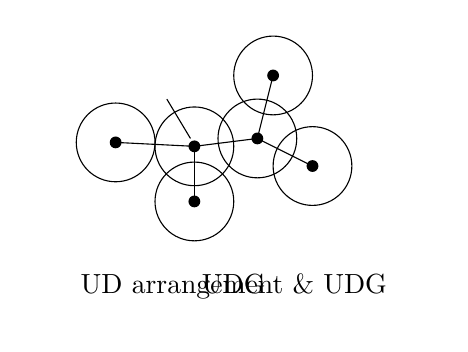
\begin{tikzpicture}[scale=0.5]
    \
    \coordinate (V) at (2,2);
    \coordinate (V2) at (3.6,2.2);
   \newcommand{\None}{(2,0.6),(0,2.1),(V2)}
   \newcommand{\Ntwo}{(5,1.5),(4,3.8)}

   \uncover{  
   	\fill (V) circle(0.15);
	\foreach \coord in \None{\fill \coord circle(0.15);}
	\foreach \coord in \Ntwo{\fill \coord circle(0.15);}
	\foreach \coord in \None{\draw (V) --\coord;}
	\foreach \coord in \Ntwo{\draw (V2) --\coord;}
	
}        
   \uncover{
	 \draw (V) circle(1);
   	 \foreach \coord in \None{\draw \coord circle(1);}
	\foreach \coord in \Ntwo{\draw \coord circle(1);}
}        
\uncover{\draw[] ($(V)+(-0.10,0.2)$)--+(-0.6,1)node[above]{$\vv$};}       
\coordinate(CAP) at (3,1);
\node<1> [below=1cm, align=flush center,text width=5cm] at (CAP){UDG};
\node [below=1cm, align=flush center,text width=5cm] at (CAP){UD arrangement \& UDG};
\draw[white] (-1.4,5) rectangle(7.2,-2.5);\end{tikzpicture}
\begin{tikzpicture}[scale=0.5]
    \coordinate (V) at (2,2);
    \coordinate (V2) at (3.6,2.2);
   \newcommand{\None}{(2,0.6),(0,2.1),(V2)}
   \newcommand{\Ntwo}{(5,1.5),(4,3.8)}

      
   \uncover{

	\foreach \coord in \None{\fill[gray!50] \coord circle(0.15);}
	\foreach \coord in \Ntwo{\fill[gray!50] \coord circle(0.15);}
	\foreach \coord in \None{\draw[gray!50] (V) --\coord;}
	\foreach \coord in \Ntwo{\draw[gray!50] (V2) --\coord;}
   	 \foreach \coord in \None{\draw[gray!50] \coord circle(1);}
	\foreach \coord in \Ntwo{\draw[gray!50] \coord circle(1);}
     	\fill[] (V) circle(0.15);
     	\draw[thick] (V) circle(1);	
}   

   \uncover{  


\draw[ultra thick,darkred] (V) circle(0.25);
}  

\coordinate(CAP) at (3,1);
 \node<3> [below=1cm, align=flush center,text width=5cm] at (CAP){$N_0$};
 \node [below=1cm, align=flush center,text width=5cm] at (CAP){$N_0$ (black) and $I_0$ (red)};
\draw[white] (-1.4,5) rectangle(7.2,-2.5);\end{tikzpicture}
\\
    \begin{tikzpicture}[scale=0.5]
    \
    \coordinate (V) at (2,2);
    \coordinate (V2) at (3.6,2.2);
   \newcommand{\None}{(2,0.6),(0,2.1),(V2)}

   \newcommand{\Ntwo}{(5,1.5),(4,3.8)}
  
   \uncover{
	\draw<5>[thick] (V) circle(1);
   	\draw[thick,gray!50] (V) circle(1);       
	\foreach \coord in \Ntwo{\draw[gray] \coord circle(1);}
	\foreach \coord in \None{\draw[thick] \coord circle(1);}
	\foreach \coord in \Ntwo{\draw[gray] (V2) --\coord;}
	\foreach \coord in \None{\draw (V) --\coord;}
   	\fill (V) circle(0.15);
}    
\foreach \coord in \Ntwo{\draw[thick] (V2) --\coord;}
\foreach \coord in \None{\draw[thick] (V) --\coord;}
\foreach \coord in \None{\draw[ultra thick,darkred] \coord circle(0.25);}
\foreach \coord in \None{\fill[] \coord circle(0.15);}
\foreach \coord in \Ntwo{\fill[gray!50] \coord circle(0.15);}

\coordinate(CAP) at (3,1);
\node<5> [below=1cm, align=flush center,text width=5cm] at (CAP){$N_1$};
\node [below=1cm, align=flush center,text width=5cm] at (CAP){$N_1$ and $I_1$}; 
\draw[white] (-1.4,5) rectangle(7.2,-2.5);\end{tikzpicture}
\begin{tikzpicture}[scale=0.5] % i guess this is the bist picture of them all. use this for copypasting later
\coordinate (V) at (2,2);
\coordinate (V2) at (3.6,2.2);
\newcommand{\None}{(2,0.6),(0,2.1),(V2)}
\newcommand{\Nonee}{(2,0.6),(0,2.1)}
\newcommand{\Ntwo}{(5,1.5),(4,3.8)}

\draw<7>[thick] (V) circle(1);
\draw<7>[thick] (V2) circle(1);
\foreach \coord in \Ntwo{\fill \coord circle(0.15);}
\foreach \coord in \None{\fill \coord circle(0.15);}
\draw[thick,gray!50] (V) circle(1);
\draw[thick,gray!50] (V2) circle(1);
\foreach \coord in \Nonee{\draw[thick] \coord circle(1);}
\foreach \coord in \Ntwo{\draw[thick] \coord circle(1);}
\foreach \coord in \Ntwo{\draw[thick] (V2) --\coord;}
\foreach \coord in \None{\draw[thick] (V) --\coord;}
\foreach \coord in \Nonee{\draw[ultra thick,darkred] \coord circle(0.25);}
\foreach \coord in \Ntwo{\draw[ultra thick,darkred] \coord circle(0.25);}
\fill<7> (V) circle(0.15);
\fill<7> (V2) circle(0.15);
\fill[gray] (V) circle(0.15);
\fill[gray] (V2) circle(0.15);
\coordinate(CAP) at (3,1);
\node<7> [below=1cm, align=flush center,text width=5cm] at (CAP){$N_2$};
\node<8> [below=1cm, align=flush center,text width=5cm] at (CAP){$N_2$ and $I_2$};
\node [below=1cm, align=flush center,text width=5cm] at (CAP){$N_2$ and $I_2$, $\bar r = 1$};
\draw[white] (-1.4,5) rectangle(7.2,-2.5);
\end{tikzpicture}
\end{frame}



\begin{frame}
From the definition of $N_r$ it follows that for the subgraph $G' = G[N_{\bar r+1}]$ the maximum independent set size is bounded:
\begin{align*}
\alpha(G') \leq \rho|I_{\bar r}|.
\end{align*}
$H = G\setminus G'$ has no vertices adjacent to vertices in $N_{\bar r}$ and therefore a $\rho$-approximate IS for $H$ ($I_H$) combined with $I_{\bar r}$ yields a $\rho$-approximate IS for G.
\begin{align*}
\alpha(G) \leq \alpha(H) + \alpha(G') \leq \rho|I_H \cup I_{\bar r}|
\end{align*}
\end{frame}

\begin{frame}
\frametitle{Algorithm}
\begin{enumerate}
\item Define sets $N_r$ for arbitary node $v \in V$ and calculate independent sets $I_r$ until stopping criterion reached
\begin{itemize}
\item Remember that $r$ has constant bound $\implies$ determining $I_r$ is possible in $O(n^{C^2})$.
\end{itemize}
\item Repeat step 1. for subgraph $H= G \setminus N_{\bar r +1}$ until $H = \varnothing$.
\item Output independent set $I = \bigcup I_{\bar r}$ where $I_{\bar r}$ are alle the IS found in step 1. 
\end{enumerate}
\end{frame}

\subsection{Weighted MIS}
\begin{frame}
\frametitle{Algorithm for maximum weighted independent set problem}
%\begin{itemize}
When defining sets $N_r$ start with $v$ such that 
\begin{align*}
\omega(v) \geq \omega(v') \forall v' \in V \qquad (=\text{argmax } \omega(v)) 
\end{align*}and use
\begin{align*}
\omega(I_{r+1}) > \rho \omega(I_r)
\end{align*}as stopping criterion (for $\bar r$) to get bound on the weight of the IS of the subsets.
%\end{itemize}
\end{frame}

\section{MIS for Rectangles}
\subsection{MIS for arbitrary rectangles}
\begin{frame}
\frametitle{MIS for arbitrary rectangles \cite{agarwallabel}}
\begin{itemize}
\item Geometric objects are rectangles in $\mathbb R^2$ with parallel edges
\item Desired: Biggest subset of those rectangles that don't intersect each other
\item $\log n$ -- approximate algorithm for this case with $O(n\log n)$ runtime: 
\begin{itemize}
\item Divide and concquer: Split into subsets and calculate independent sets for them
\item Combine IS of subsets.
\end{itemize}
\end{itemize}
\end{frame}

\begin{frame}
\frametitle{Maximum independent set for arbitrary rectangles}
Given: Set $S$ of rectangles.
\begin{itemize}
\item Sort edges by $x$ and $y$ coordinates --- $O(n\log n)$
\item \begin{enumerate}
\item Find median in $x$ coordinate --- $O(n)$
\item Divide rectangles in 3 sets: $S_M$ (intersecting median), $S_L$ and $S_R$ (left and right of median)
\item Apply algorithm 1-4 recursively to $S_L$ and $S_R$ if their size is $\geq 2$ to get approximate solution, else calculate MIS in $O(1)$.
\item Calculate MIS of $S_M$ with greedy approach (outlined on blackboard) --- $O(n)$
\item Take either $I_L \cup I_R$ or $I_M$ 
\end{enumerate}
\end{itemize}

\uncover{Overall runtime: $O(n\log n)$}
\end{frame}
%\item TODO: create slides for algorithm in \cite{agarwallabel}.
%\item Algorithm is more or less: sort edges of rectangles, find median, subdivide in rectangles on left and right side of meidan and combine their IS with those of  rectangles intersectiong median.
%\item Uses the known height of rectangles combined with their y coordinate to reduce problem difficulty by seperating into set of easier problems ($\rightarrow$ dynamic programming)


\subsection{MIS for unit height rectangles}
\begin{frame}
\frametitle{MIS for unit height rectangles \cite{agarwallabel}}
\begin{itemize}]
\item Map labels often have similar/identical height
%\item Could be exploited for better results
\item Use height to split problem in small subproblems that don't depend on each other
\item Apply greedy scheme from before for subproblems
\end{itemize}
\end{frame}

\begin{frame}
\frametitle{MIS for unit height rectangles (UHR)}
\uncover{Draw $m+1$ horizontal lines that fulfill the following criteria:
\begin{itemize}
\item $y$ - distance $>1$
\item Each line intersects $\geq 1$ rectangles
\item Each rectangle is intersected by $1$ line.
\end{itemize}
}
\uncover{Solve MIS for subsets $S_0$ to $S_m$ (one for every line) with greedy algorithm.\\[1em]}
\uncover{Take union of either odd or even subsets}
\end{frame}

%\begin{frame}
%\frametitle{Possible improvements:}
%\end{frame}

\subsection{Take away points}
\begin{frame}
\frametitle{Take away points}
For difficult problems use all available information about objects at hand to make problem solvable (or at least get good approximate solutions):
\begin{itemize}
\item 1st algorithm (UDG): minimum area of a independent set of geometric shapes used to get an upper bound on size of subsets 
\item 2nd algorithm (greedy heuristic): reduce dimensionality of problem by line that intersects all rectangles
\item 3rd algorithm (UHR): decompose problem into subproblems that can be solved easily
\end{itemize}

\end{frame}




%\section*{Stuff}
%\subsection{References}
\begin{frame}[allowframebreaks]\frametitle{References}

\end{frame}

\begin{frame}
\frametitle{Remarks I}
Robustness of PTAS for M(W)IS on UDG
\begin{itemize}
\item Polynomial runtime only possible on UDG \uncover{as it assumes bounded area of IS with given size}
\item UDG are subset of all graphs --- proving that graph is UDG is \NP- hard
\item Robustness would mean: Determine in polynomial runtime whether runtime will be polynomial. \uncover{Is this possible?}
\item Actually possible in this case:  If $|I_r > (2r+1)^2$ is found $\implies$ graph is not UDG.
\end{itemize}
\end{frame}

\begin{frame}
\frametitle{Remarks II}
Improving PTAS for unit height rectangles to {$(1+\varepsilon)$-- approximative} scheme:
\begin{itemize}]
\item Algorithm described solves $n$ independent subproblems optimally and discards results of $\frac{n}{2}$
\item Discard solutions of subproblems that are boundaries of used solutions
\item Could be improved by solving bigger subproblems with less discarded ``boundary-problems'' in between
\item Solving subproblems of $k$ lines each only every $\frac{1}{k}$-th subproblem has to be discarded $\rightarrow$ $\left(1+\frac{1}{k}\right)$-- approximation.
\end{itemize}
\end{frame}
\end{document}



